\documentclass[11pt]{article}
	\usepackage{listings}
	\usepackage{amsmath}
	\usepackage{amssymb}
	\usepackage[usenames,dvipsnames,svgnames,table]{xcolor}
	\usepackage[hidelinks=true]{hyperref}
	\usepackage{parskip}
	\usepackage{indentfirst}
	\usepackage{graphicx}
	\usepackage{tikz}
	\usetikzlibrary{arrows.meta, positioning}
	
	\setlength{\parindent}{2em} % Ajusta el valor 2em según tus preferencias

	
	% BEGIN CUSTOM PYTHON
	% Fuente para python
	\DeclareFixedFont{\ttb}{T1}{txtt}{bx}{n}{11} % for bold
	\DeclareFixedFont{\ttm}{T1}{txtt}{m}{n}{11}  % for normal

	% Mis colores
	\definecolor{deepblue}{rgb}{0,0,0.5}
	\definecolor{deepred}{rgb}{0.6,0,0}
	\definecolor{deepgreen}{rgb}{0,0.5,0}

	% Python style for highlighting
	\newcommand\pythonstyle{\lstset{
	language=Python,
	basicstyle=\ttm,
	breakatwhitespace=false,         % Activarlo para que los saltos automáticos solo se apliquen en los espacios en blanco
  	breaklines=true,                 % Activa el salto de línea automático
  	tabsize=2,	                   % Establece el salto de las tabulaciones a 2 espacios
  	numbers=left,					% Pone el numero de lineas
	morekeywords={self},              % Add palabras que se pintan de azul
	keywordstyle=\ttb\color{deepblue},
	emph={DiffieHellman, compartir_clave_publica, generar_clave_secreta, __generarClaves__, __init__, compartir_clave_secreta, cifrar_xor, descifrar_xor},          % Add palabras que se pinten de rojo
	emphstyle=\ttb\color{deepred},    % Custom highlighting style
	stringstyle=\color{deepgreen},
	frame=tb,                         % Recuadro
	showstringspaces=false
	}}


	% Comando para escribir python directamente en el .tex
	\lstnewenvironment{python}[1][]
	{
	\pythonstyle
	\lstset{#1}
	}
	{}

	% Comando para escribir python desde un fichero externo
	\newcommand\pythonexternal[2][]{{
	\pythonstyle
	\lstinputlisting[#1]{#2}}}

	% Comando para escribir codigo suelto python en una linea
	\newcommand\pythoninline[1]{{\pythonstyle\lstinline!#1!}}
	% END CUSTOM PYTHON

    \title{\textbf{\huge Intercambio de claves de Diffie y Hellman}}
    \author{Adrián Racero Serrano\\Juan Manuel Cardeñosa Borrego}
    \date{}
    

    
    \addtolength{\topmargin}{-3cm}
    \addtolength{\textheight}{3cm}
    
\renewcommand{\contentsname}{Índice}

\begin{document}
\maketitle

\thispagestyle{empty}

\newpage

\setcounter{page}{1}
\tableofcontents

\newpage

\section{Introducción}
El algoritmo Diffie-Hellman debe su nombre a sus creadores Whitfield Diffie y Martin Hellman. Creado en 1976, es uno de los protocolos de intercambio de claves más antiguos que todavía se siguen usando en la actualidad. Sus creadores fueron galardonados con el premio A.M. Turing 2015 por este trabajo, con el que revolucionaron por completo la seguridad informática.

Este algoritmo permite a dos usuarios cualesquiera intercambiar, de forma confidencial, una clave secreta $K$ (o de sesión) para posteriormente cifrar de forma simétrica los mensajes entre ellos dos.

El funcionamiento de este algoritmo es más sencillo de lo que parece y se usa frecuentemente en protocolos y aplicaciones de encriptado de datos, como SSL (Secure Sockets Layer), SSH (Secure Shell) o VPN (Virtual Private Network). Este algoritmo permite que dos entidades (A y B) puedan generar una clave $K_{AB}$ de forma simultánea, y sin enviarla por el canal de comunicaciones.

\section{Algoritmo}
1) A y B necesitan establecer y compartir valores comunes, como un valor \textit{q} primo y una raíz primitiva $\alpha$  de $q$:

Para todo primo $q$ existe un elemento $\alpha \in (\mathbb{Z}/q\mathbb{Z})^{\times}$ con $\text{ord}(\alpha) = q - 1 = \phi(q) =  \# (\mathbb{Z}/q\mathbb{Z})^{\times}$.
$(\mathbb{Z}/q\mathbb{Z})^{\times}$ es el grupo multiplicativo de las clases de equivalencia módulo $q$, es decir, que no tienen ningún factor primo en común con $q$:
\begin{center}
$(\mathbb{Z}/q\mathbb{Z})^{\times} = \{1, \alpha, \alpha^2, \ldots, \alpha^{q-2}\}$.\\
\end{center}

Este $\alpha$ se llama una \textbf{raíz primitiva} módulo $q$. Ejemplo: para $q = 5$, $\alpha = 3$ es una raíz primitiva módulo 5, ya que:
$3^0 \mod 5 = 1$, $3^1 \mod 5 = 3$, $3^2 \mod 5 = 4$ y $3^3 \mod 5 = 2$.

2) Tanto A como B generan sus claves privadas ($X_{A/B}$) y públicas ($Y_{A/B}$) teniendo en cuenta que:  $ Y_{A} \equiv \alpha^{X_A} \pmod{q}$, donde $0 \le X_A \le (q-1)$, $X_A$ es el logaritmo discreto de $Y_A$, y se representa $dlog_{\alpha,q}$ ($Y_A$). Por tanto, la efectividad del algoritmo depende de la dificultad de computar logaritmos discretos.

3) Tanto A como B comparten sus respectivas claves públicas ($Y_A$/$Y_B$).

4) Tanto A como B generan la clave de sesión: 
\begin{center}
$K_{AB} = (Y_B)^{X_A} \mod q \rightarrow K_{AB} = (\alpha^{X_B})^{X_A} \mod q$  \\
$K_{AB} = (Y_A)^{X_B} \mod q \rightarrow K_{AB} = (\alpha^{X_A})^{X_B} \mod q$  \\
\end{center}

A y B generan la misma clave secreta sin necesidad de compartir sus claves privadas:

\begin{center}
$K_{AB} = \alpha^{X_B X_A} \mod q = \alpha^{X_A X_B} \mod q$
\end{center}

El siguiente diagrama de secuencia representa la interacción entre dos entidades A y B durante el intercambio de claves:
\begin{center}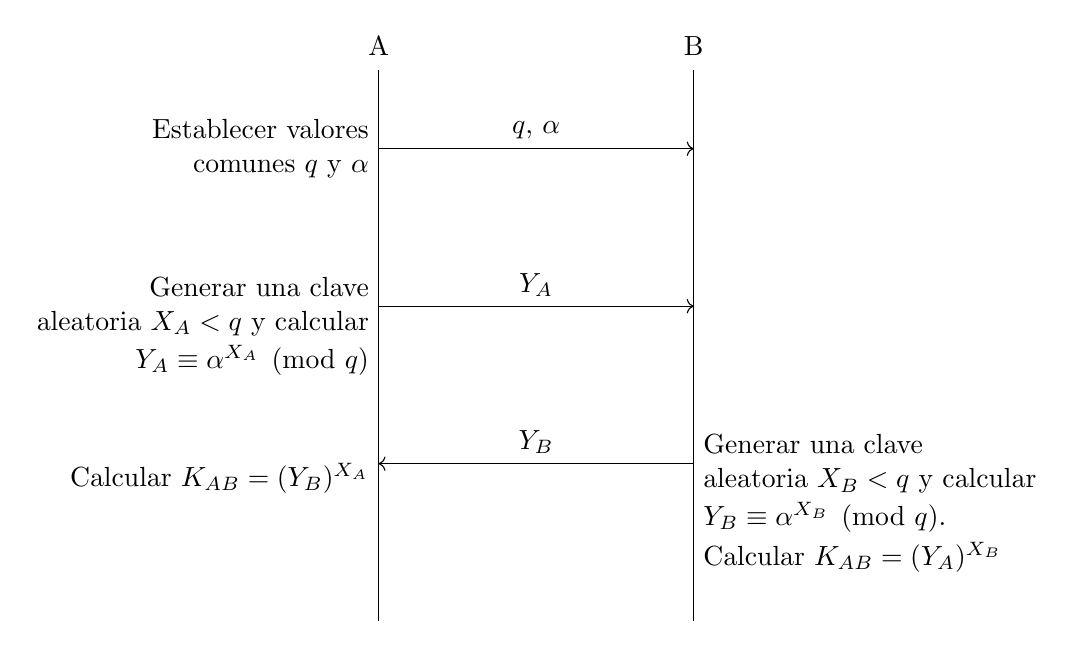
\begin{tikzpicture}
    \draw (-2,0) -- (-2,-7) (2,0) -- (2,-7);
    \node at (-2,.3) {A};
    \node at (2,.3) {B};
    \draw[->] (-2,-1) node[left,above left] {Establecer valores} -- node[midway,above] {$q$, $\alpha$} (2,-1);
    \draw (-2,-1.5) node[left, above left] {comunes $q$ y $\alpha$};
    \draw[->] (-2,-3) node[left,above left] {Generar una clave} -- node[midway,above] {$Y_A$} (2,-3);
    \draw (-2,-3.5) node[left, above left] { aleatoria $X_A < q$ y calcular};
    \draw (-2,-4) node[left, above left] { $Y_{A} \equiv \alpha^{X_A} \pmod{q}$};
    \draw[<-] (-2,-5) -- node[midway,above] {$Y_B$} (2,-5) node[right,above right] {Generar una clave};
    \draw (2,-5.5) node[right, above right] { aleatoria $X_B < q$ y calcular};
    \draw (2,-6) node[right, above right] { $Y_{B} \equiv \alpha^{X_B} \pmod{q}.$};
    \draw (2,-6.5) node[right, above right] {Calcular $K_{AB} = (Y_A)^{X_B}$};
	\draw (-2,-5.5) node[left, above left] { Calcular $K_{AB} = (Y_B)^{X_A}$};
\end{tikzpicture}\end{center}

\section{Difusión y confusión}

Claude Shannon introdujo los conceptos de "confusión" y "difusión" como dos principios fundamentales en la teoría de la información y la criptografía. Aunque estos conceptos son fundamentales en el diseño de cifradores simétricos, como los utilizados en la criptografía de clave secreta, no se aplican directamente al intercambio de claves de Diffie-Hellman, que está más relacionado con la criptografía de clave pública y problemas matemáticos específicos.

Estos conceptos se aplican una vez obtenida la clave secreta en el algoritmo, para mayor seguridad durante el intercanbio de mensajes.

\begin{itemize}
	\item \textbf{Confusión:} Implica hacer que la relación entre el texto cifrado y la clave sea compleja y difícil de entender. Esto se logra mediante operaciones no lineales y sustituciones, complicando la relación entre el texto cifrado y la clave.

	\item \textbf{Difusión:}: Busca dispersar la influencia de un bit de entrada en muchos bits de salida. Pequeños cambios en la entrada deben propagarse a través del cifrado, distribuyendo la información en el texto cifrado. Es decir, cada carácter del texto cifrado ha de depender de diferentes partes de la clave.
\end{itemize}

\section{Autenticación}

En el mundo real, el intercambio de claves Diffie-Hellman rara vez se utiliza por sí solo. La razón principal detrás de esto es que no proporciona autenticación, lo que deja a los usuarios vulnerables a los ataques de intermediarios.

Estos ataques pueden tener lugar cuando el intercambio de claves Diffie-Hellman se implementa por sí mismo, porque no tiene forma de verificar si la otra parte en una conexión es realmente quien dice ser. Sin ninguna forma de autenticación, los usuarios pueden conectarse con atacantes cuando creen que se están comunicando con una parte de confianza.

Por esta razón, el intercambio de claves Diffie-Hellman generalmente se implementa junto con algunos medios de autenticación. Esto a menudo implica el uso de certificados digitales y un algoritmo de clave pública, como RSA, para verificar la identidad de cada parte.


\section{Problemas de seguridad del intercambio de claves Diffie-Hellman}
La seguridad del intercambio de claves Diffie-Hellman depende de cómo se implemente, así como de los números que se elijan para ello. Como dijimos anteriormente, no tiene medios para autenticar a la otra parte por sí misma, pero en la práctica se utilizan otros mecanismos para garantizar que la otra parte en una conexión no sea un impostor.

\subsection {El ataque de Logjam}

El intercambio de claves Diffie-Hellman se diseñó sobre la base de que el problema del logaritmo discreto era difícil de resolver. El mecanismo conocido públicamente más eficaz para encontrar la solución es el algoritmo de tamiz de campo numérico (método utilizado para encontrar números primos en un rango específico).

Las capacidades de este algoritmo se tuvieron en cuenta cuando se diseñó el intercambio de claves Diffie-Hellman. En 1992, se sabía que para un grupo dado, G, tres de los cuatro pasos involucrados en el algoritmo podrían potencialmente calcularse de antemano. Si se guardara este progreso, el paso final podría calcularse en un tiempo comparativamente corto. Esto no fue demasiado preocupante hasta que se descubrió que una parte significativa del tráfico de Internet utiliza los mismos grupos que son de 1024 bits o menos. En 2015, un equipo académico ejecutó los cálculos para el primo de 512 bits más común utilizado por el intercambio de claves Diffie-Hellman en TLS.

También pudieron degradar el 80$\%$ de los servidores TLS que admitían DHE-EXPORT, de modo que aceptaran un intercambio de claves Diffie-Hellman de grado de exportación de 512 bits para la conexión. Esto significa que cada uno de estos servidores es vulnerable a un ataque de un adversario con recursos suficientes.

Los investigadores continuaron extrapolando sus resultados, estimando que un estado-nación podría romper un primo de 1024 bits. Al romper el número primo de 1024 bits más utilizado, el equipo académico estimó que un adversario podría monitorizar el 18$\%$ del millón de sitios web HTTPS más populares.

Continuaron diciendo que un segundo principal permitiría al adversario descifrar las conexiones del 66$\%$ de los servidores VPN y del 26$\%$ de los servidores SSH. Más adelante en el informe, los académicos sugirieron que es posible que la NSA ya tenga estas capacidades.

A pesar de esta vulnerabilidad, el intercambio de claves Diffie-Hellman aún puede ser seguro si se implementa correctamente. Mientras se use una clave de 2048 bits, el ataque Logjam no funcionará. Los navegadores actualizados también están a salvo de este ataque.

\section{Variaciones del intercambio de claves Diffie-Hellman}

El intercambio de claves Diffie-Hellman se puede implementar de distintas maneras y también proporciona la base para varios otros algoritmos. Algunas de estas implementaciones proporcionan autorización, confidencialidad, técnicas criptográficas varias, como el \emph{Perfect forward secrecy}, ...

\subsection{Curva elíptica Diffie-Hellman}
Curva elíptica Diffie-Hellman aprovecha la estructura algebraica de las curvas elípticas, lo que permite que su implementación alcance niveles similares de seguridad con tamaños de clave más pequeños. Las claves de curva elíptica de 224 bits proporcionan el mismo nivel de seguridad que las claves RSA de 2048 bits. Esto mejora la eficiencia de conmutación y reduce los requisitos de almacenamiento.

Diffie-Hellman de curva elíptica funciona de manera similar al intercambio de claves estándar Diffie-Hellman, excepto por la longitud de clave más pequeña y su naturaleza basada en curva elíptica.

\subsection{TLS}

TLS, un protocolo utilizado para proteger gran parte de Internet, puede utilizar los intercambios Diffie-Hellman de tres formas diferentes: anónima, estática y efímera. En la práctica, sólo debería implementarse la ley Diffie-Hellman efímera, ya que otras opciones tienen problemas de seguridad.


\begin{itemize}
    \item \textbf{Diffie-Hellman anónimo:} no utiliza ninguna autenticación y la deja vulnerable a los ataques \emph{man-in-the-middle}. No debe usarse ni implementarse.
    \item \textbf{Static Diffie-Hellman:} utiliza certificados para autenticar el servidor. No autentica al cliente de forma predeterminada, ni proporciona \emph{Perfect forward secrecy}.
    \item \textbf{Diffie-Hellman efímero:} se considera la implementación más segura porque proporciona un secreto directo perfecto. Se  suele combinar con un algoritmo como DSA o RSA para autenticar a una o ambas partes en la conexión. Esta versión utiliza diferentes pares de claves cada vez que se ejecuta el protocolo. Esto le da a la conexión un \emph{Perfect forward secrecy}, porque incluso si una clave se ve comprometida en el futuro, no se puede usar para descifrar todos los mensajes pasados.\\
\end{itemize}


\section{El intercambio de claves Diffie-Hellman y RSA}

El intercambio de claves Diffie-Hellman se complementa a menudo con algoritmos como RSA para proporcionar autenticación en conexiones seguras. RSA, aunque capaz de cifrar mensajes, se utiliza principalmente para autenticar a las partes mediante certificados digitales verificados por autoridades de certificación. Este proceso implica la firma de mensajes con claves privadas y la verificación con las claves públicas correspondientes en los certificados.

A pesar de la autenticación lograda por RSA, su uso exclusivo para cifrar todas las comunicaciones sería ineficiente. Por lo tanto, muchos protocolos de seguridad optan por combinar el intercambio de claves Diffie-Hellman para llegar a un secreto compartido eficientemente. Este secreto, a menudo utilizado como clave simétrica compartida, se emplea en algoritmos de cifrado simétrico como AES para la transmisión segura de datos entre las partes autenticadas.

Este enfoque es más eficiente que depender únicamente de RSA para todo el intercambio, ya que el cifrado de clave simétrica es más rápido. Además, RSA presenta desventajas adicionales, como la necesidad de relleno para seguridad y la falta de secreto directo perfecto en comparación con el intercambio efímero de Diffie-Hellman.

En lugar de RSA, el intercambio de claves Diffie-Hellman puede combinarse con algoritmos como el Estándar de firma digital (DSS) para proporcionar autenticación, intercambio de claves, confidencialidad e integridad de datos, eliminando la necesidad de RSA en determinadas situaciones. Este enfoque flexible se adapta a las necesidades específicas de seguridad en las conexiones.


\section{Computación cuántica en el intercambio de claves Diffie-Hellman}

La computación cuántica, una disciplina en constante evolución, plantea desafíos significativos en el ámbito de la criptografía. Los detalles exactos de su funcionamiento son complejos, pero se espera que los ordenadores cuánticos tengan la capacidad de resolver problemas que actualmente son demasiado difíciles para las ordenadores clásicos, lo que abre nuevas posibilidades y riesgos.

La amenaza principal se encuentra en los algoritmos cuánticos, como el algoritmo de Grover, que podrían acelerar los ataques contra sistemas de cifrado que utilizan claves simétricas. Aunque este riesgo puede mitigarse duplicando el tamaño de la clave, la preocupación se centra en el algoritmo de Shor, que afectaría directamente a la criptografía de clave pública.

Los algoritmos de clave pública comunes, como Diffie-Hellman, se basan en la complejidad de problemas como el logaritmo discreto y la factorización de enteros. Con el avance de las computadoras cuánticas, se espera que el algoritmo de Shor simplifique la resolución de estos problemas, poniendo en peligro la seguridad de los sistemas criptográficos que dependen de ellos.

En particular, el intercambio de claves Diffie-Hellman se sustenta en la dificultad práctica de resolver el problema del logaritmo discreto con la tecnología actual. Aunque no hay una línea de tiempo precisa sobre cuándo la computación cuántica representará una amenaza seria para este protocolo, se están desarrollando sustitutos y alternativas en la criptografía para anticipar y contrarrestar estos posibles riesgos. La seguridad de la criptografía de clave pública, fundamental para proteger las comunicaciones, es el foco principal de estos desafíos que los criptógrafos están abordando activamente.

\section{Conclusión}
En conclusión, el intercambio de claves de Diffie-Hellman ha demostrado ser una piedra angular en la construcción de comunicaciones seguras en entornos digitales. A lo largo de décadas, este protocolo ha ofrecido una solución eficaz para el desafío fundamental de establecer claves compartidas en un canal inseguro.

La gran característica del intercambio de claves de Diffie-Hellman radica en su capacidad para garantizar la confidencialidad de las claves compartidas, incluso en un escenario donde un atacante puede interceptar la comunicación. Su enfoque basado en la complejidad computacional de los logaritmos discretos ha resistido la prueba del tiempo, proporcionando una base sólida para numerosos protocolos de seguridad.

Sin embargo, es crucial reconocer las limitaciones inherentes del Diffie-Hellman, especialmente en lo que respecta a la autenticación. En el mundo real, su implementación a menudo se combina con certificados digitales y algoritmos de clave pública para abordar la falta de verificación de la identidad de las partes involucradas. Esta adaptación ha permitido que el Diffie-Hellman se integre con éxito en protocolos como TLS/SSL, proporcionando una seguridad más completa y autenticada.

A medida que la ciberseguridad evoluciona, el intercambio de claves de Diffie-Hellman enfrentará desafíos continuos, desde la amenaza potencial de la computación cuántica hasta la necesidad constante de mejorar los protocolos de autenticación. Sin embargo, su impacto duradero en la seguridad de la información subraya su importancia como un pilar confiable en la construcción de sistemas de comunicación seguros y confiables. En un panorama digital en constante cambio, el Diffie-Hellman sigue siendo un contribuyente fundamental a la garantía de la privacidad y la integridad de las comunicaciones en línea.


\section{Bibliografía}

\emph{https://cadadr.org/teoria-de-numeros-basica/hoja-6.pdf}

\emph{https://ciberseguridad.com/guias/recursos/intercambio-claves-diffie-hellman/}

\emph{https://www.computerweekly.com/es/definicion/Intercambio-de-claves-Diffie-Hellman-intercambio-de-claves-exponencial}


\newpage
\section{Anexo}
\subsection{Código}
La clase \pythoninline{DiffieHellman}: \\
\pythonexternal{code/algoritmo.py}
\ \\
Ejecucion del algoritmo:
\pythonexternal{code/ejecucion.py}
\ \\
Salida de la ejecución: \\
\lstinputlisting{code/salida.txt}

\end{document}









